
\section{Introduction}
\par

Shallow Water Equations model the propagation of disturbances in water and other incompressible fluids and are used to describe the 
dynamics of important phenomenon like tsunami.The underlying assumption is that the depth of the fluid is small compared to 
the wave length of the disturbance. The conservative form of the shallow water equations is,

\begin{equation}\label{eqn:1}
{\frac{\partial h}{\partial t} + \frac{\partial (hu)}{\partial x} + \frac{\partial (hv)}{\partial y} = 0 } \notag
\end{equation}
\begin{equation}
{\frac{\partial (hu)}{\partial t} + \frac{\partial (hu^2 + \frac{1}{2} gh ^2)}{\partial x} + \frac{\partial (huv)}{\partial y} = fhv }
\end{equation}
\begin{equation}
{\frac{\partial (hv)}{\partial t} + \frac{\partial (huv)}{\partial x}+\frac{\partial (hv^2 + \frac{1}{2} gh ^2)}{\partial y}=-fhu } \notag
\end{equation}

Here $h$ $\ge$ 0 is the fluid height, $u$ and $v$ are the horizontal and vertical velocities, $g$ is the acceleration due to gravity (9.8m/s2 on Earth) 
and $f$ is the Coriolis force. We let


\[U = \begin{bmatrix} h \\ hu \\ hv\end{bmatrix},\,\, F(U) = \begin{bmatrix} hu \\ hu^2 +  \frac{1}{2} gh^2 \\ huv \end{bmatrix},\,\,
G(U) = \begin{bmatrix} hv \\ huv \\ hv2 +  \frac{1}{2} gh^2 \end{bmatrix},\,\, 
S(U) = \begin{bmatrix} 0 \\ fhv \\ -fhu \end{bmatrix}, \]


which can now be rewritten in a more compact form,
\begin{equation}
 {\frac{\partial U}{\partial t} + \frac{\partial F(U)}{\partial x} + \frac{\partial G(U)}{\partial y} = S(U) } \label{eqn:2}
 \end{equation}

 
In the absence of the Coriolis force, we get the standard form of the conservation law,
\begin{equation}
{\frac{\partial U}{\partial t} + \frac{\partial F(U)}{\partial x} + \frac{\partial G(U)}{\partial y} = 0 } \label{eqn:3}
\end{equation}
We specify either periodic boundary condition, or ``free boundary'' conditions for $h$ and ``reflective'' boundary conditions for $uh$ and $uv$.
Free boundary conditions mean the boundary exerts no stress, while reflective boundary conditions mean the boundary behaves like a mirror.

\section{1D Solver}
\par Consider the shallow water equations in one dimension,

\begin{equation}
\frac{\partial U}{\partial t} + \frac{\partial F(U)}{\partial x} = 0,
\end{equation}

where $U = [h, hu]^T$ and $F(U) = [hu,\,\, hu^2 + \frac{1}{2} + gh^2]^T$. Define $q(x,t) = u(x,t) h(x,t)$ so we have

\[U = \begin{bmatrix} h, \\ q\end{bmatrix},\,\, F(U) = \begin{bmatrix} q,\\ \frac{q^2}{h} + \frac{1}{2} gh^2 \end{bmatrix}.\]

Let $A$ be a Jacobian of $F(U)$. Thus

\begin{equation}
A = \begin{bmatrix} 0 & 1 \\ -\frac{q^2}{h^2} + gh & \frac{2q}{h}\end{bmatrix}
\end{equation}

with eigenvalues $\lambda = \frac{q}{h} \pm \sqrt{gh}.$ Since $h(x,t) > 0$ and $g$ is a positive constant eigenvalues of the Jacobian are
real and distinct (i.e A has full set of eigenvectors). Hence, the system is hyperbolic. \newline

The Lax-Wendroff method for equation (4) is,
\begin{equation}\label{eqn:4}
U_i^{n+1}=U_i^n-\frac{{\Delta t}}{2}((I-\frac{{\Delta t}}{{\Delta x}}A_{i+1/2}^n)(D_+F_i^n)+((I+\frac{{\Delta
t}}{{\Delta x}}A_{i-1/2}^n)(D_{\_}F_i^n).
\end{equation}
where \(F_i^n=F(U_i^n), A_{i+1/2}\) is the Jacobian matrix of F evaluated at \(U_{i+1/2}\) and \(D_+\) and \(D_-\) are the standard forward
and backward difference operators defined as,
\begin{equation}\label{eqn:5}
D_{\pm }w(x)=\frac{\pm w(x\pm {\Delta x})-\pm w(x))}{{\Delta x}}. 
\end{equation}

Assuming we have \(N_x\) points in the x-direction with \(\Omega =[0\;1]\), and \(1\leq i\leq n\), periodic boundary
conditions can be imposed by \(U_1=U_{N_x}\), reflective boundary conditions at\(x=0\) by \(U_1=-U_2\), and free boundary conditions at \(x=0\) by
\(U_1=U_2\). These equations describe how conditions are imposed on the entire vector U, here we implement reflective boundary
conditions for hu and free boundary conditions for h. The intial conditions are chosen to be interesting, such that $h=4+sin(2$pi$x)$ for $u=0$, and
 $h=e^{-(\frac{x-\mu }{\sigma })^2}for \; u=0$. \newline

\begin{figure}[htp]
    \centering
    \begin{subfigure}[b]{0.312\textwidth}
        \centering
        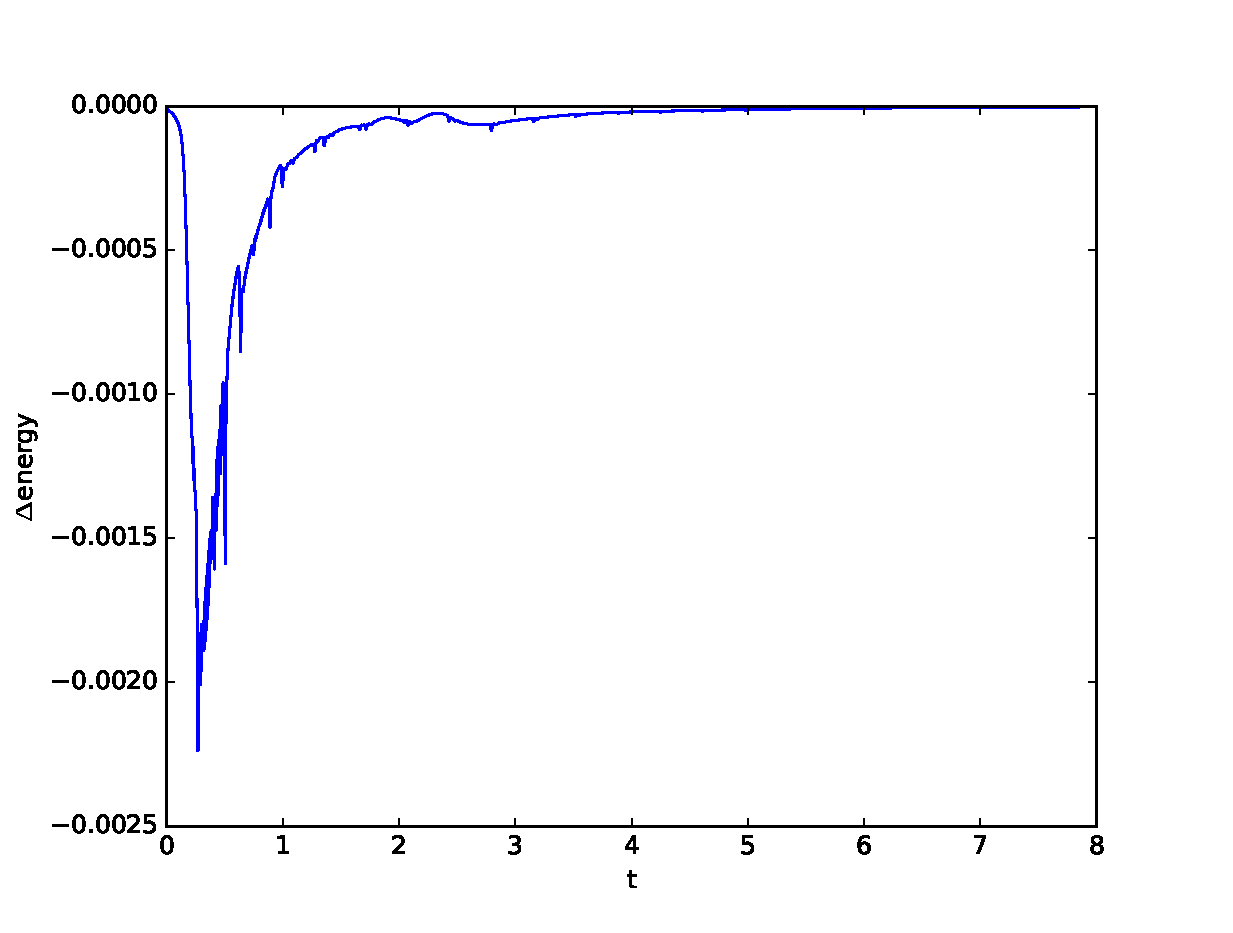
\includegraphics[width=\textwidth]{images/E1d.eps}\hfill
        \caption{Energy}
        \label{fig:Energy}
    \end{subfigure}
    \hfill
    \begin{subfigure}[b]{0.32\textwidth}
        \centering
        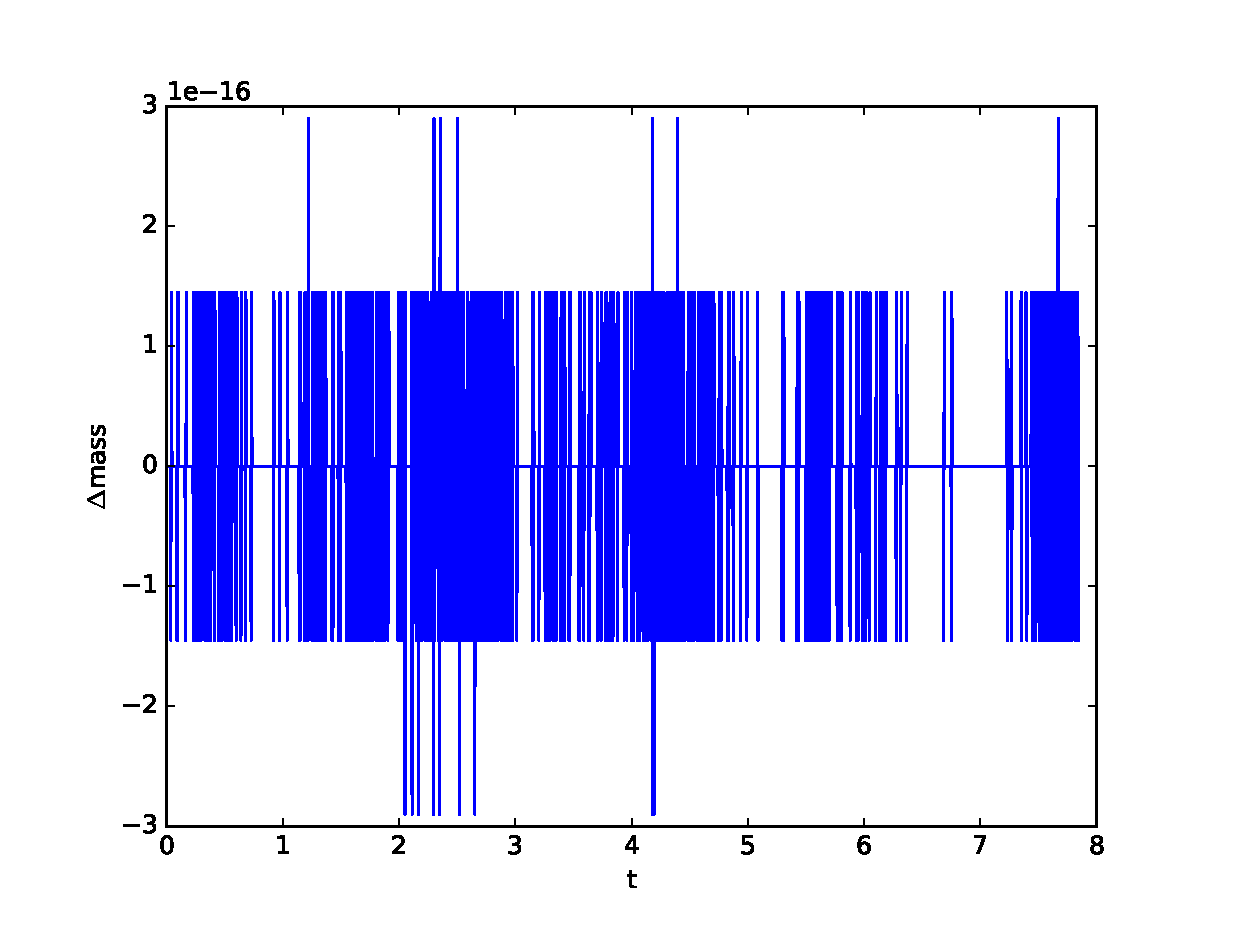
\includegraphics[width=\textwidth]{images/Ma1d.eps}\hfill
        \caption{Mass}
        \label{fig:Mass}
    \end{subfigure}
    \hfill
    \begin{subfigure}[b]{0.32\textwidth}
        \centering
        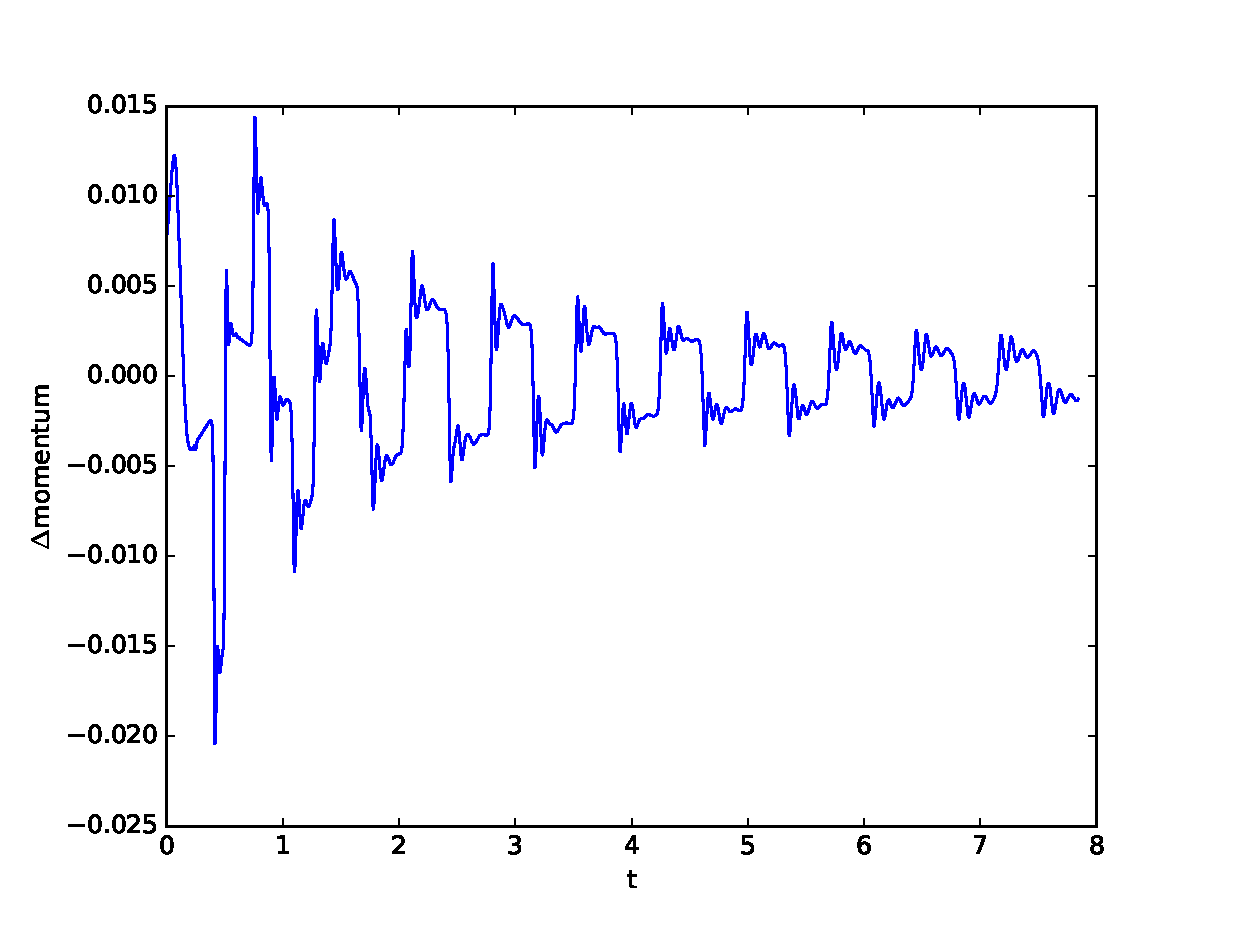
\includegraphics[width=\textwidth]{images/Mo1d.eps}\hfill
        \caption{Momentum}
        \label{Momentum}
    \end{subfigure}
    \caption{1D conservation plots.}
    \label{fig:three graphs}
\end{figure}

\section{2D Solver}
\subsection{1D Conservation Laws}
We expect the following quantities to be conserved: mass h, momentum or mass velocity, $hu$ and $hv$, and
energy 0.5($hv^2$+$gh^2$). Potential vorticity is only looked at in the 2D solver. Invesigation of conservation of momentum in solver.
 Is the momentum conserved, what explanation do we have?

TO DO 1D FIGURES!!!



The spatial domain for the 2D solver is \(\Omega =[{  }1]\times [{  }1].\) To go about solving the system in 2D there are many options,
we compare two schemes. Lax-Wendfoff, and a two step version of Richtmeyer proposed. \newline
\newline

\subsection{Dimensional Splitting (Lax Wendroff)}

Using the 1D equations of the Lax-Wendroff scheme for system (4) a dimenional split can be implemented by 
doing a step in $x$, followed by a step in $y$: 
\begin{equation}\label{eqn:6}
U_{i,j}^* = U_{i,j}^n - \frac{\Delta t}{2} (( I- \frac{\Delta t}{\Delta x} A_{i+1/2,j}^n ) D_+^xF_{i,j}^n + (I+ \frac{\Delta
t}{\Delta x} A_{i-1/2,j}^n) D_{\_}^xF_{i,j}^n)
\end{equation}
\begin{equation}\label{eqn:7}
U_{i,j}^{n+1} = U_{i,j}^* - \frac{\Delta t}{2} B(I - \frac{\Delta t}{\Delta y} B_{i,j+1/2}^*) D_+^yG_{i,j}^*) +(I + \frac{\Delta
t}{\Delta x} B_{i,j-1/2}^* ) D_{\_}^y F_{i,j}^* )
\end{equation}
\newline


\subsection{Two-Step Lax-Wendroff Method (Richtmeyer)}

Richtmeyer proposed a two-step version of the Lax-Wendroff method, which is much simpler than the original, especially in multi-dimensional problems.
The first step uses Lax's  method and the second step is a midpoint leapfrog calculation. 

\begin{equation}\label{eqn:8}
U_{i}^{n+1} = \frac{1}{2}(U_{i+1}^{n}+U_{i-1}^{n})-\Delta{t} \Big(\frac{F_{i+1}^{n}-F_{i-1}^{n}}{2\Delta x}\Big)
\end{equation}
\begin{equation}\label{eqn:9}
U_{i}^{n+2} = U_{i}^{n} + (2\Delta t) \Big ( \frac{ F_{i+1}^{n+1}-F_{i-1}^{n+1} }{ 2 \Delta x } \Big)
\end{equation} 
\newline

The values $F_{i \pm 1}^{n+1}$ in the second step are based on the $U_{i \pm 1}^{n+1}$ results on the first step. The first step is considered
a provisonal step, with signifigance attached only to the results of the second step in each sequence. This method does not look anything like the original
Lax-Wendroff method of \eqref{eqn:6}, but substitution of \eqref{eqn:10} and \eqref{eqn:11} shows that the methods are equivalent. 
\newline
The extension to multiple dimensions is obvious and neat.
\begin{equation}\label{eqn:10}
\frac{\partial U}{\partial t} = - \Big( \frac{\partial F}{\partial x} + \frac{\partial G}{\partial y} \Big)
\end{equation}

\begin{dmath}\label{eqn:11}
U_{i}^{n+1} = \frac{1}{4} \Big( U_{i+1,j}^{n} + U_{i-1,j}^{n} + U_{i,j+1}^{n} + U_{i,j-1}^{n} \Big) 
- (\Delta t) \Big( \frac{ F_{i+1,j}^{n} - F_{i-1,j}^{n} }{2 \Delta x}  + \frac{ G_{i,j+1}^{n} - G_{i,j-1}^{n} }{ 2 \Delta x }  \Big)
\end{dmath} 

This 2D-scheme requires about a fourth of the computational time as the original Lax-Wendroff method, and produces less shock overshoot than the orignal. 
\newline

The boundary conditions are prescribed for two cases. The first, periodic for both $h$, $hu$, and $hv$, and the second,
 and more complicated conditions, free for $h$, reflective in the horizontal direction and free in the vertical direction 
for $uh$, and reflective in the vertical direction and free in the horizontal direction for $vh$. The initial conditions are then
 chosen to be piecewise, 

\begin{equation}\label{eqn:12}
u_0(x,y)=
\begin{array}{ll}
\Big\{ & 
\begin{array}{ll}
 8, & \text{if} (x-0.3)^2+(y-0.3)^2 \\
 1, & \text{otherwise} \\
\end{array}
\end{array}
\end{equation}

interestingly forming a cylindrical column.


\begin{figure}[htp]
    \centering
    \begin{subfigure}[b]{0.46\textwidth}
        \centering
        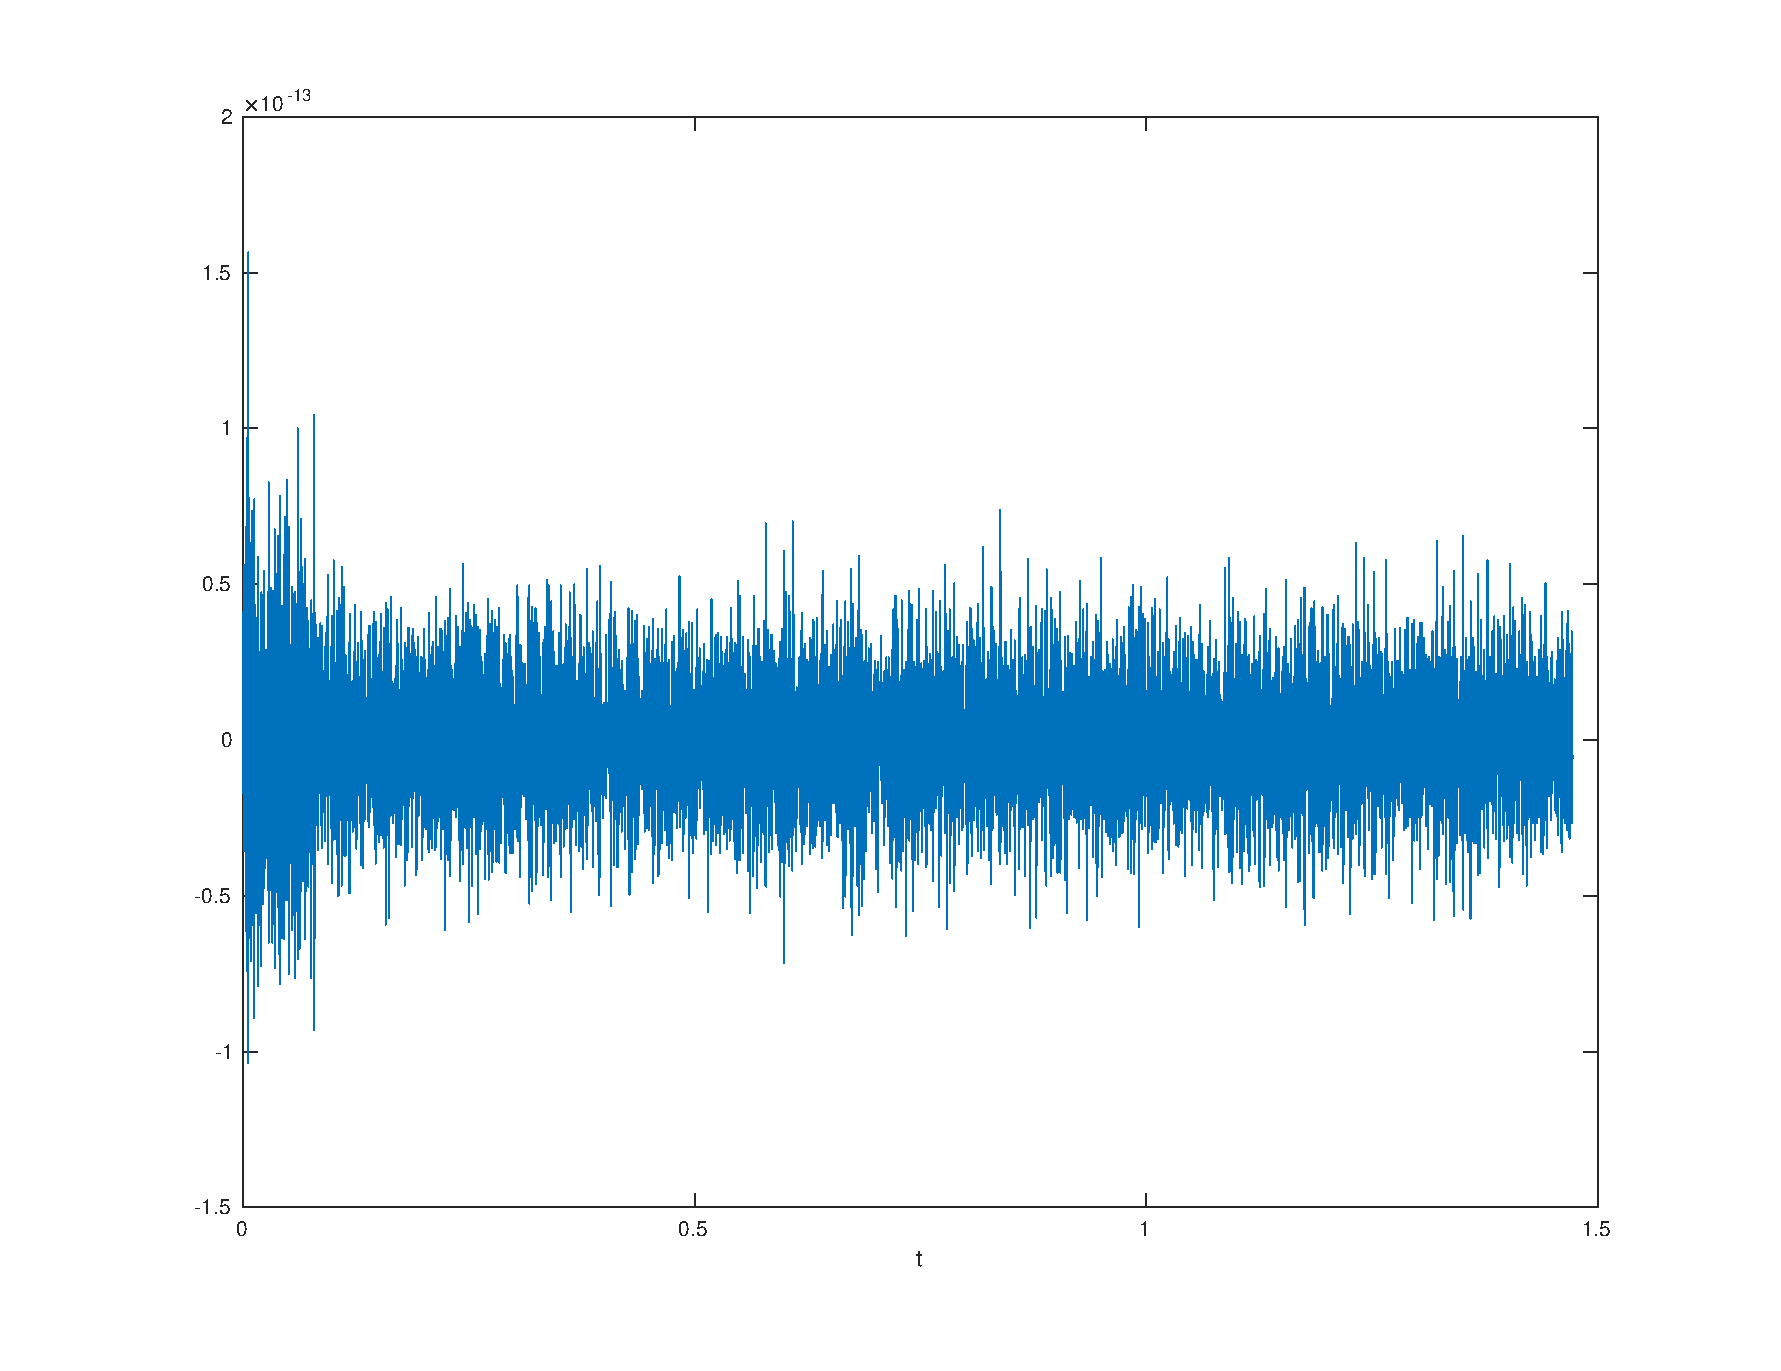
\includegraphics[width=\textwidth]{images/cons_mass.eps}\hfill
        \caption{Energy}
        \label{fig:Energy}
    \end{subfigure}
    \hfill
    \begin{subfigure}[b]{0.45\textwidth}
        \centering
        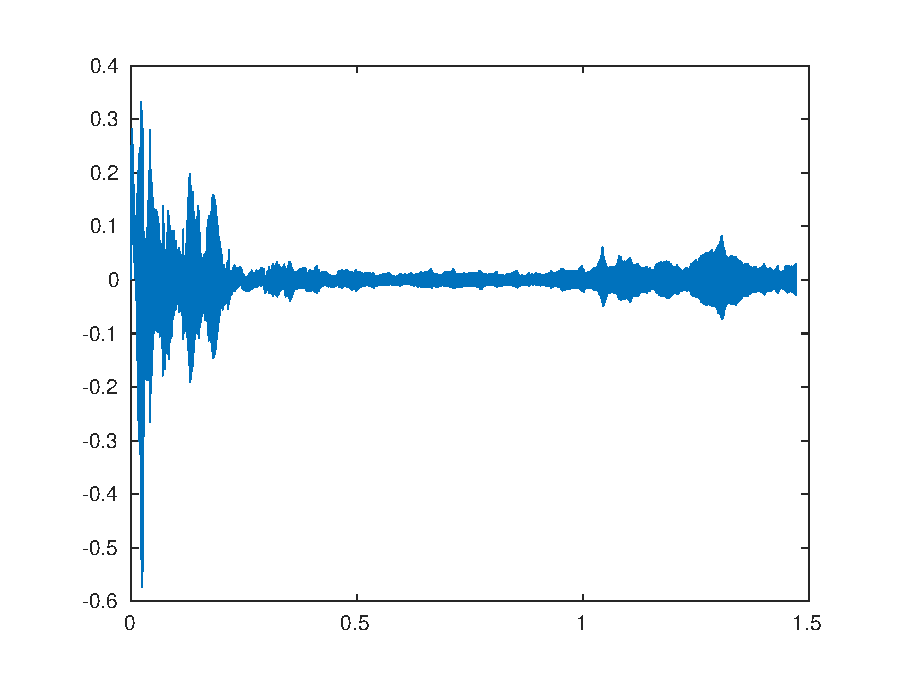
\includegraphics[width=\textwidth]{images/cons_energy.eps}\hfill
        \caption{Mass}
        \label{fig:Mass}
    \end{subfigure}
    \caption{2d conservation plots for mass, and energy.}
    \label{fig:three graphs}
\end{figure}

\begin{figure}[htp]
    \centering
    \begin{subfigure}[b]{0.3\textwidth}
        \centering
        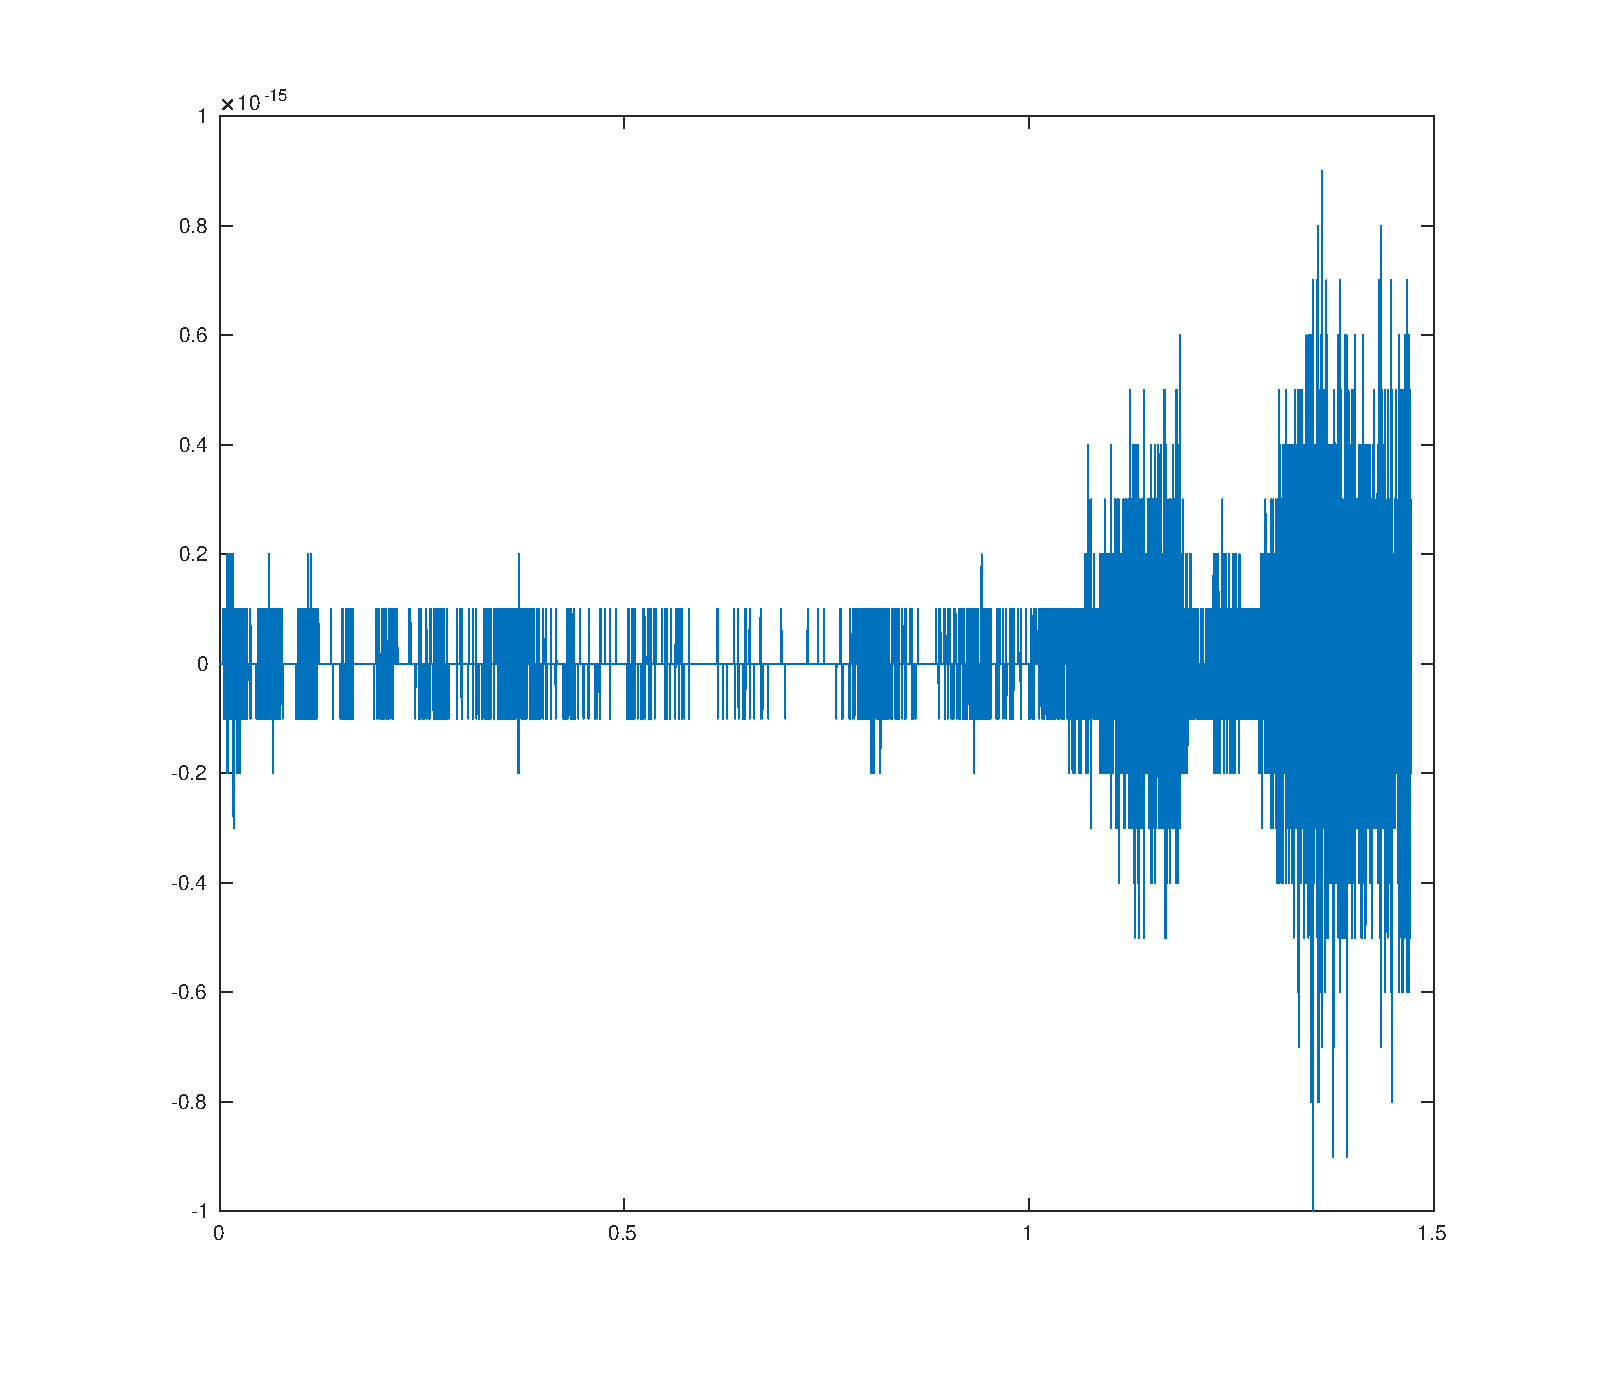
\includegraphics[width=\textwidth]{images/cons_momu.eps}\hfill
        \caption{u-momentum}
        \label{fig:Energy}
    \end{subfigure}
    \hfill
    \begin{subfigure}[b]{0.3\textwidth}
        \centering
        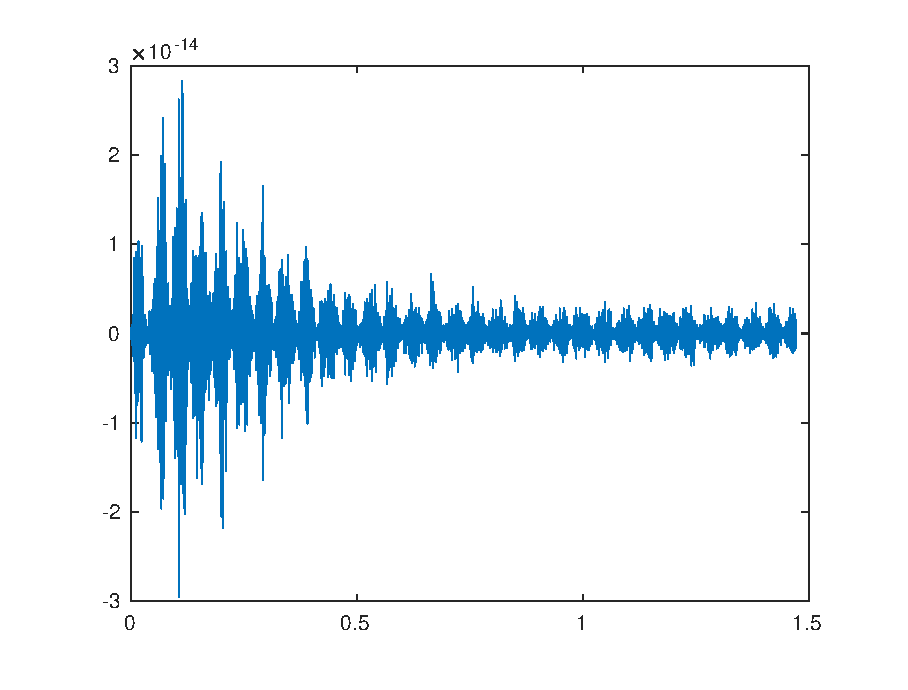
\includegraphics[width=\textwidth]{images/cons_momv.eps}\hfill
        \caption{v-momentum}
        \label{fig:Mass}
    \end{subfigure}
    \hfill
    \begin{subfigure}[b]{0.3\textwidth}
        \centering
        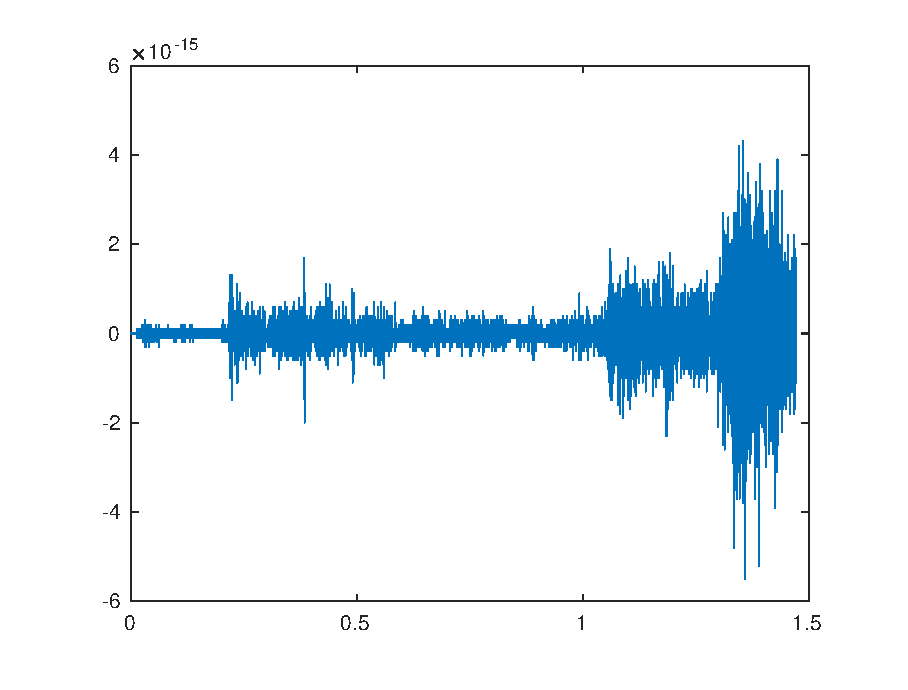
\includegraphics[width=\textwidth]{images/cons_vort.eps}\hfill
        \caption{vorticity}
        \label{Momentum}
    \end{subfigure}
     \hfill
    \caption{2D Conservation plots.}
    \label{fig:three graphs}
\end{figure}

Lorem ipsum dolor sit amet, ad vix saperet mediocrem consetetur, ut admodum torquatos maiestatis est, 
no aeque singulis interpretaris sea. Ut paulo petentium eum, eum id malorum dignissim. Sed ex modus quodsi. 
Simul commodo scribentur ne has, mei ei dico interpretaris. Iriure tibique gloriatur vim an. Mea ea idque 
fabulas lucilius.

Vel timeam fuisset te. Duo ea nobis omnium pericula, sed discere scripserit ei, mea an illud dolore adolescens.
 Eu cum eligendi voluptatum, brute lobortis eam an, ea mei fastidii complectitur. An causae accusam pri. 
 In ius possit oportere.ges:


%%%%%%%%%%%%%%%%%%%%%%%%%%%%%%%%%%%%%%%%%%%%%%%%%%%%%%%%%%%%%%%%%%%%%%%
%Bibiography

\begin{thebibliography}{1}

\bibitem{Leveque}  Leveque, R. J. {\\Finite Volume Methods for Hyperbolic Problems} 2002:
Cambridge University Press, N.Y.

\bibitem{Roach} Roach, P. J. {\\Computational Fluid Dynamics} 1985: Hermosa Publishers. Albuquerque, N.M.

\bibitem{fo} Bob Tadashi Wakabayashi {\em Anti-Foreignism and Western
Learning in Early-Modern Japan} 1986: Harvard University Press.

\end{thebibliography}